\documentclass[journal]{IEEEtran}
\usepackage[a5paper, margin=10mm, onecolumn]{geometry}
\usepackage{amsmath,amssymb,amsfonts}
\usepackage{graphicx}
\usepackage{enumitem}
\usepackage{hyperref}

\begin{document}

\title{11.16.3.7}
\author{EE24BTECH11004 - Ankit Jainar}
\maketitle

\textbf{Question:}
Three coins are tossed once. Find the probability of getting exactly two tails.

\section*{Theoretical Solution}
The sample space for tossing three coins is:
\begin{align}
    S = \{HHH, HHT, HTH, HTT, THH, THT, TTH, TTT\}
\end{align}
The total number of outcomes is:
\begin{align}
    |S| = 8
\end{align}
The favorable outcomes (exactly two tails) are:
\begin{align}
    A = \{HTT, THT, TTH\}
\end{align}
The number of favorable outcomes is:
\begin{align}
    |A| = 3
\end{align}
The probability of getting exactly two tails is:
\begin{align}
    P(A) = \frac{|A|}{|S|} = \frac{3}{8} = 0.375
\end{align}
\section*{Theoretical Solution Using Z-Transform}
To solve the problem using the Z-transform, we first define the random variable \( X \) to represent the number of tails. The probability mass function (PMF) for a single coin toss is:
\begin{align}
    P(X = 0) &= 0.5, \quad P(X = 1) = 0.5.
\end{align}
For three independent coin tosses, the generating function using the Z-transform is:
\begin{align}
    G(z) = (0.5 + 0.5z)^3.
\end{align}
Expanding \( G(z) \) gives the following:
\begin{align}
    G(z) &= 0.125 + 0.375z + 0.375z^2 + 0.125z^3.
\end{align}
Thus, the probability mass function of the number of tails \( Y \) is:
\begin{align}
    P(Y = k) = \begin{cases} 
    0.125, & k = 0, \\
    0.375, & k = 1, \\
    0.375, & k = 2, \\
    0.125, & k = 3.
    \end{cases}
\end{align}

The probability of getting exactly two tails is:
\begin{align}
    P(\text{exactly two tails}) = P(Y = 2) = 0.375.
\end{align}

\section*{Introduction}
This task involves simulating the random tossing of three coins using a C program, compiling it into a shared object (.so) file, and using Python to process the results and generate a probability distribution plot.

\section*{C Code Description}
The C program generates random samples for the coin tosses, where the outcomes are categorized based on the number of tails. The program uses the \texttt{rand()} function to simulate the random tosses and increments a counter for each outcome with exactly two tails.

\section*{Python Code Description}
The Python code performs the following:
\begin{enumerate}
    \item Loads the shared object file generated from the C program using the \texttt{ctypes} library.
    \item Simulates a specified number of random coin tosses (e.g., 1,000,000 trials).
    \item Calculates the probability of getting exactly two tails using the formula:
    \begin{align}
    P(\text{exactly two tails}) = \frac{\text{frequency of exactly two tails}}{\text{total trials}}
    \end{align}
    \item Plots the probability distribution using \texttt{matplotlib}.
\end{enumerate}

\section*{Graphical Output}
The Python code generates a bar chart where:
\begin{itemize}
    \item The x-axis represents the outcomes: "0 tails", "1 tail", "2 tails", and "3 tails".
    \item The y-axis represents the probabilities, ranging from 0 to 1.
    \item The bar height for "2 tails" corresponds to the probability $P(A) = 0.375$.
\end{itemize}

\subsubsection*{Probability Mass Function (PMF)}
The PMF represents the probability of each individual outcome in the sample space \( S \). For the coin toss:
\begin{align}
S = \{0 \text{ tails}, 1 \text{ tail}, 2 \text{ tails}, 3 \text{ tails}\},
\end{align}

The PMF is extracted by looking at the coefficients of powers of \( z \) in the expansion of \( G(z) \). This corresponds to the probability of obtaining \( k \) tails, where \( k = 0, 1, 2, 3 \). From the expansion:
\[
G(z) = 0.125 + 0.375z + 0.375z^2 + 0.125z^3,
\]
we can directly read off the probabilities:

\[
P(X = 0) = 0.125, \quad P(X = 1) = 0.375, \quad P(X = 2) = 0.375, \quad P(X = 3) = 0.125.
\]

Thus, the PMF is:
\[
P(X = k) = \begin{cases}
0.125 & \text{for } k = 0, \\
0.375 & \text{for } k = 1, \\
0.375 & \text{for } k = 2, \\
0.125 & \text{for } k = 3, \\
0 & \text{otherwise}.
\end{cases}
\]
\subsection*{CDF (Cumulative Distribution Function)}
The CDF is obtained by summing up the probabilities from the PMF up to a given value \( k \). The CDF, \( F(x) \), is defined as:
\[
F(x) = P(X \leq x) = \sum_{k \in S, k \leq x} P(X = k).
\]
We calculate the CDF at the points \( x = 0, 1, 2, 3 \):

- For \( x = 0 \) (0 tails):
\[
F(0) = P(X \leq 0) = P(X = 0) = 0.125.
\]

- For \( x = 1 \) (1 tail):
\[
F(1) = P(X \leq 1) = P(X = 0) + P(X = 1) = 0.125 + 0.375 = 0.5.
\]

- For \( x = 2 \) (2 tails):
\[
F(2) = P(X \leq 2) = P(X = 0) + P(X = 1) + P(X = 2) = 0.125 + 0.375 + 0.375 = 0.875.
\]

- For \( x = 3 \) (3 tails):
\[
F(3) = P(X \leq 3) = P(X = 0) + P(X = 1) + P(X = 2) + P(X = 3) = 0.125 + 0.375 + 0.375 + 0.125 = 1.
\]

Thus, the CDF is:
\[
F(x) = \begin{cases}
0 & \text{for } x < 0, \\
0.125 & \text{for } 0 \leq x < 1, \\
0.5 & \text{for } 1 \leq x < 2, \\
0.875 & \text{for } 2 \leq x < 3, \\
1 & \text{for } x \geq 3.
\end{cases}
\]

\subsection*{Simulation Process}
We simulate the tossing of three coins using the following steps:
\begin{enumerate}
    \item The sample space consists of outcomes in the set:
    \begin{align}
    S = \{0 \text{ tails}, 1 \text{ tail}, 2 \text{ tails}, 3 \text{ tails}\}.
    \end{align}
    \item For each simulated toss, a random integer \( X \) is generated such that:
    \begin{align}
    X \in \{0, 1, 2, 3\},
    \end{align}
    using a random number generator function based on binomial trials.
    \item The number of occurrences of each outcome is tracked over \( N \) trials, where \( N \) is the total number of simulations.
    \item Both the PMF and CDF are computed:
    \begin{itemize}
        \item PMF: The frequency of each outcome is divided by the total number of trials to comput the probabilities.
        \item CDF: The cumulative probabilities are calculated as the running total of the PMF values.
    \end{itemize}
\end{enumerate}

\subsection*{Calculation of Probabilities}
\subsubsection*{Probability of Exactly Two Tails (PMF)}
The probability of exactly two tails is computed as:
\begin{align}
P(\text{exactly two tails}) = \frac{3}{8} = 0.375.
\end{align}

\subsubsection*{Cumulative Probability (CDF)}
The cumulative probability of outcomes up to a given value is:
\begin{align}
F(x) = 
\begin{cases} 
P(0 \text{ tails}), & x = 0 \text{ tails}, \\
P(0 \text{ tails}) + P(1 \text{ tail}), & x = 1 \text{ tail}, \\
P(0 \text{ tails}) + P(1 \text{ tail}) + P(2 \text{ tails}), & x = 2 \text{ tails}, \\
1, & x = 3 \text{ tails}.
\end{cases}
\end{align}
For the coin toss:
\begin{align}
F(0 \text{ tails}) = 0.125, \quad F(1 \text{ tail}) = 0.5, \quad F(2 \text{ tails}) = 0.875, \quad F(3 \text{ tails}) = 1.
\end{align}

\subsubsection*{Probability of Selecting \( X \notin S \)}
Since all outcomes belong to the set \( S = \{0, 1, 2, 3\}\), the probability of selecting \( X \notin S \) is:
\begin{align}
P(X \notin S) = 0.
\end{align}

\subsection*{Output Representation}
The computed probabilities are represented in two forms:
\begin{itemize}
    \item PMF: The probabilities of each outcome (0 tails, 1 tail, 2 tails, 3 tails).
    \item CDF: The cumulative probabilities up to each outcome.
\end{itemize}

\section*{Conclusion}
This task demonstrates the integration of C and Python for simulating and visualizing a probabilistic experiment. The probability of getting exactly two tails from tossing three coins is calculated as \textbf{0.375}, matching the theoretical value.

\begin{figure}[h!]
   \centering
   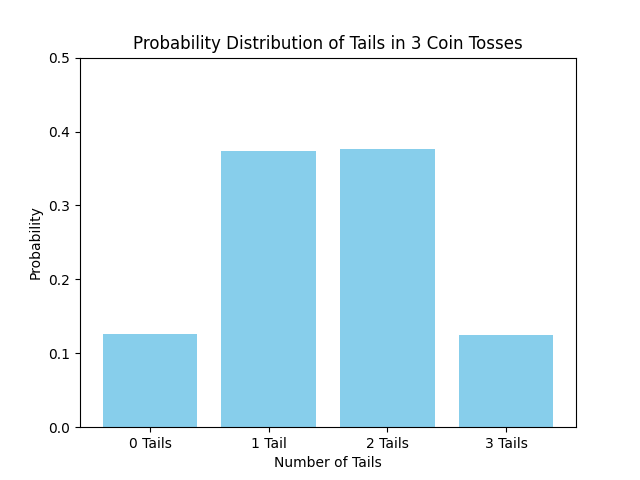
\includegraphics[width=\columnwidth]{figs/fig1.png}
   \end{figure}
\begin{figure}[h!]
   \centering
   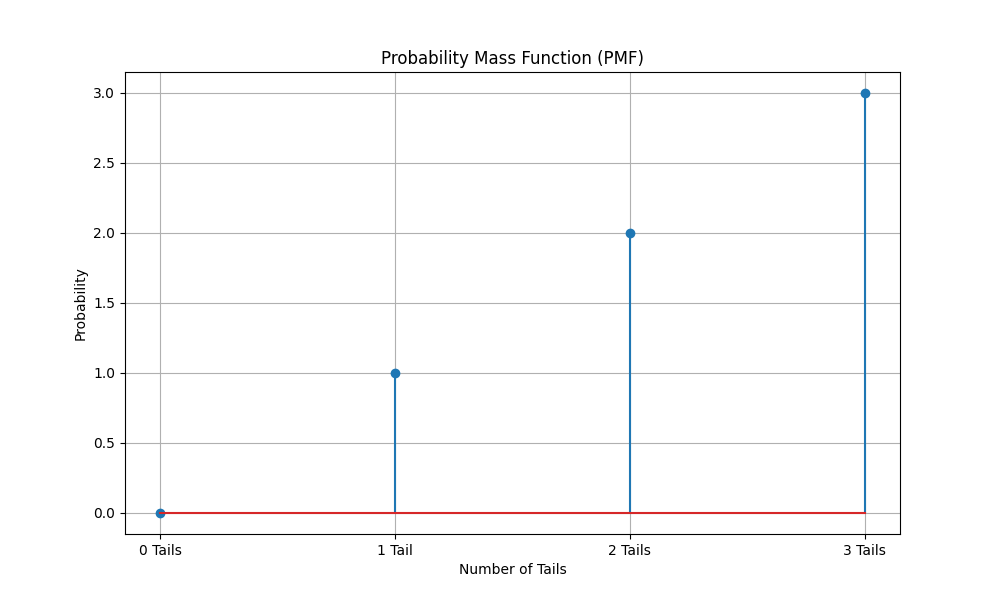
\includegraphics[width=\columnwidth]{figs/fig2.png}
   \end{figure}
\begin{figure}[h!]
   \centering
   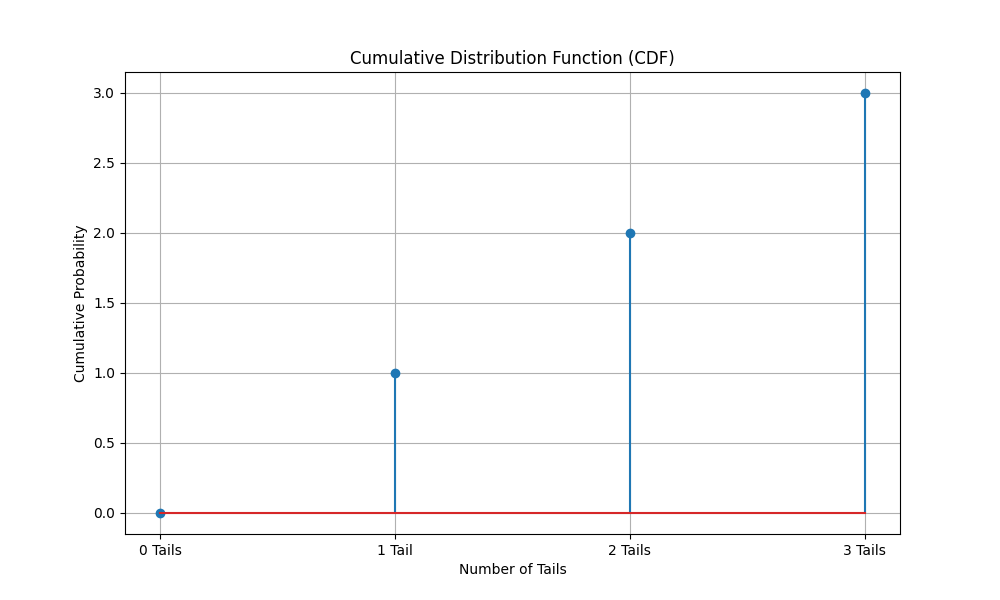
\includegraphics[width=\columnwidth]{figs/fig3.png}
   \end{figure}
\begin{figure}[h!]
   \centering
   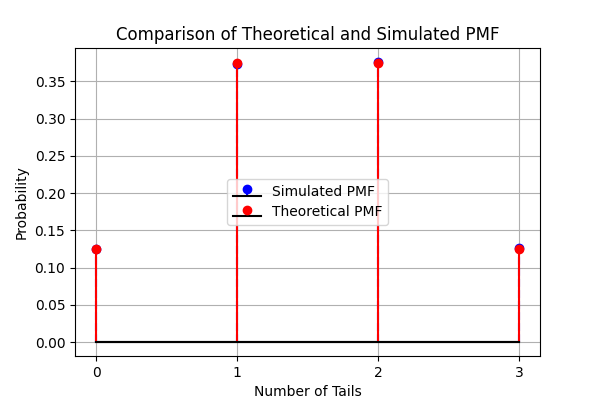
\includegraphics[width=\columnwidth]{figs/fig4.png}
   \end{figure}
\end{document}

